\documentclass[10pt,pdf,hyperref={unicode}]{beamer}


% \documentclass[aspectratio=43]{beamer}
% \documentclass[aspectratio=1610]{beamer}
% \documentclass[aspectratio=169]{beamer}

\usepackage{multicol}
\usepackage{lmodern}
\usepackage{lipsum}
\usepackage{marvosym}
\usepackage{amssymb}

% подключаем кириллицу 
%\usepackage[T1,T2A]{fontenc}
\usepackage[lutf8]{luainputenc}
\usepackage[english,russian]{babel}

% отключить клавиши навигации
\setbeamertemplate{navigation symbols}{}

% тема оформления
\usetheme{CambridgeUS}
% цветовая схема
\usecolortheme{crane}

\usepackage{fontspec}
        \defaultfontfeatures{Ligatures={TeX}}
        \setmainfont{Ubuntu}
        \setsansfont{Ubuntu}
        \setmonofont{Ubuntu Mono}
    \usepackage[english,russian]{babel}

\date{}

\title[]{...ers,Developers,Developers,Developers,Dev...}   
%\subtitle{Use beamer everywhere you are}
\author[]{Кирпиченков Денис} 
\institute[]{Naumen}
%\date{\today} 
% \logo{\includegraphics[height=5mm]{images/logo.png}\vspace{-7pt}}

\begin{document}

% титульный слайд
\begin{frame}
\titlepage
\end{frame} 

\begin{frame}
\frametitle{История о разработке одного продукта} 

\begin{itemize}
\item Время разработки 10 лет
\item 3 перерождения: python, java, brand new java с GWT
\item 3 000 000 строк java-кода, 125 000 строк XML файлов,  60 000 строк скриптов
\item Комманда из 20 разработчиков
\end{itemize}

\end{frame}

\begin{frame}
\frametitle{Read,Code,Debug,Test... Repeat} 

\begin{enumerate}

	\item взять задачу;
	\item прочитать требования;
	\item реализовать;
	\item показать реализацию;
	\item отдать в тестирование;
	\item goto 1.
	
\end{enumerate}

\end{frame}

\begin{frame}
\frametitle{Что общего у (почти) всех программистов} 

\center

\includegraphics[height=0.6\textheight]{./multi_fun.png}

\end{frame}

\begin{frame}
\frametitle{void function career() \{ while(1) \{ doCodeALot() \} \} }
\framesubtitle{ обощенный путь разработчика }

Карьера разработчика:

\begin{columns}
	\column{0.5\textwidth}

		\begin{itemize}
			\item Стажер
			\item Разработчик
			\item Ведущий разработчик
			\item Главный разработчик
		\end{itemize}

	\column{0.5\textwidth}

		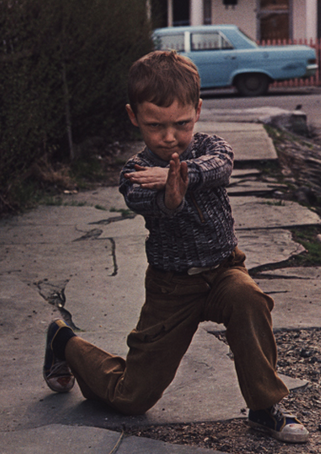
\includegraphics[width=0.5\textwidth]{./intern.png}
		
\includegraphics[width=0.484\textwidth]{./senior.png}

\end{columns}

\end{frame}

\begin{frame}
\frametitle{ Embedded решения }
\begin{columns}
	\column{0.5\textwidth}

		\begin{itemize}
			\item много итересных задач;
			\item получение уникального опыта.
		\end{itemize}

	\column{0.5\textwidth}
		\begin{itemize}
			\item довольно высокая сложность любой задачи;
			\item новые технологии и принципы разработки очень редко тут появляются.
		\end{itemize}

\end{columns}

Например, 1024 \div 2 \equiv 1024 \gg 1

\end{frame}


\begin{frame}
\frametitle{Enterprise разработка}

\begin{columns}
	\column{0.5\textwidth}
		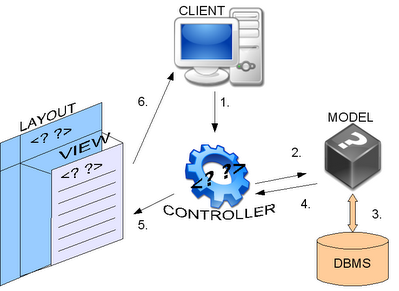
\includegraphics[width=0.8\textwidth]{./ruby.png}
	\column{0.5\textwidth}
		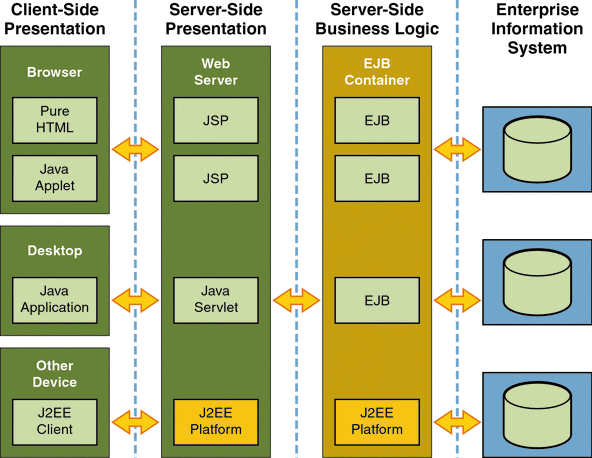
\includegraphics[width=0.8\textwidth]{./enterprise.png}
\end{columns}

\end{frame}

\begin{frame}
\frametitle{ Mobile apps }
	\center
	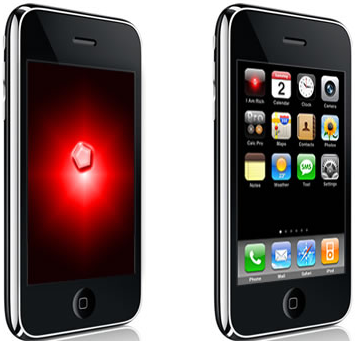
\includegraphics[width=0.4\textwidth]{./imrich.png}
\end{frame}

\begin{frame}
\frametitle{ Что нужно знать}

\begin{itemize}

	\item Язык программирования
	\item Типы данных
	\item  Особенности аппаратного обеспечения и сети

\end{itemize}

\end{frame}

\begin{frame}
\frametitle{ M x N }

\par
Есть матрица M x N. 

\par
Цель: обойти все элементы матрицы наиболее эффективным способом.

\par
Как это лучше сделать по колонка или по строкам матрицы?

\end{frame}

\begin{frame}
\frametitle{ Finale }

\center
	
\includegraphics[width=0.8\textwidth]{./run_dos_run.png}

\end{frame}

\begin{frame}
\frametitle{ Finale }

\center
	
\includegraphics[width=0.8\textwidth]{./developer.png}

\end{frame}

\end{document}